\documentclass[12pt]{beamer}
\usepackage[utf8]{inputenc}
\usepackage{lmodern}
\usepackage{german}
\usetheme{Berkeley}
\title[Semesterarbeit]{Implementation einer Win/Win Strategie für das Traveling Salesman Problem}
\author{Andreas Brönnimann}
\institute{ZHAW - Zürcher Hochschule für Angewandte Wissenschaften}
\date{11.04.2012}

\setbeamerfont{footnote}{size=\tiny}
\setbeamertemplate{footline}[frame number]
\setbeamertemplate{navigation symbols}{}

\begin{document}

    \begin{frame}
        \titlepage
    \end{frame}

    \begin{frame}
        \frametitle{Ablauf}
        \tableofcontents
    \end{frame}

    \section{Aufgabenstellung}
    \begin{frame}
        \frametitle{Aufgabenstellung}
	    \begin{itemize}
                \item Vorstellung Traveling Salesman Problem (TSP) 
                \item Vorstellung Win/Win Strategie
                \item Implementation Algorithmus
                \item Berechnung von Benchmark-Graphen
                \item Berechnung von generierten Graphen
            \end{itemize}
    \end{frame}
    \section{Traveling Salesman Problem}
    \begin{frame}
        \frametitle{Traveling Salesman Problem}
	    \begin{itemize}
                \item Problem des Handlungsreisenden
                \item kürzeste Rundreise durch n Städte
            \end{itemize}

            \begin{figure}[H]
                \centering
                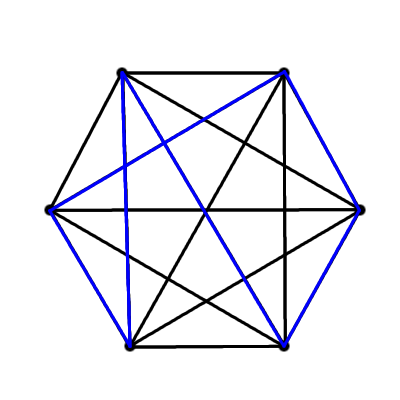
\includegraphics[width=4cm]{gfx/simple_tsp}
            \end{figure}
    \end{frame}
    \begin{frame}
        \frametitle{Traveling Salesman Problem - Geschichte}
	    \begin{itemize}
                \item 1757: Knights Tour - Leonard Euler
                \item 1930er Jahre: Forschung an der Princeton Universität
                \item 1954: 49 Städte TSP gelöst 
                \item 1977: 120 Städte TSP gelöst 
                \item 1987: 2'392 Städte TSP gelöst 
                \item 1990er Jahre: Entwicklung von Concorde
                \item 2001: 15'112 Städte TSP 
                \item 2006: 85'900 Städte TSP 
            \end{itemize}
    \end{frame}
    \section{Win/Win Strategie}
    \begin{frame}
        \frametitle{Win/Win Strategie - Grundidee}
	    \begin{itemize}
                \item zwei verwandte Probleme
                \item zwei Algorithmen
                \item Worst Case Instanzen disjunkt
            \end{itemize}
    \end{frame}
    \begin{frame}
        \frametitle{Win/Win Strategie - Anwendung TSP}
	    \begin{itemize}
                \item Traveling Salesman Problem
                \item Christofides Algorithmus
                \item Tour max. 1/2 länger als das Optimum
                    \medskip
                \item Hamiltonpfadproblem
                \item Hoogeveen Algorithmus 
                \item Tour max. 2/3 länger als das Optimum
            \end{itemize}
    \end{frame}
    \section{Algorithmus}
    \begin{frame}
    \frametitle{Algorithmus}
        \begin{scriptsize}
        \textbf{Eingabe:} Ein kompletter Graph $G = (V,E)$, eine metrische Kostenfunktion $c: E \rightarrow \mathbb{Q}^+$ und zwei Knoten $s$ und $t$.

        \begin{itemize}
            \item[1.] Minimalen Spannbaum $T$ von $G$ berechnen.
            \item[2.] Minimales Perfect Matching\footnote{für das Perfect Matching wird eine bestehende Implementation verwendet} $M_C$ der ungeraden Knoten des minimalen Spannbaumes $T$ von $G$ berechnen.
            \item[3.] Minimales Perfect Matching $M_P$ der ungeraden Knoten des Multigraphen $T$ + \{$s$, $t$\} von $G$ berechnen.
            \item[4.] Die Eulertour Eul$_C$ des Multigraphen T $\cup$ $M_C$ und den Eulerpfad Eul$_P$ des Multigraphen T $\cup$ $M_P$ berechnen.
            \item[6.] Eul$_C$ zu einer Hamiltontour $H_C$ und Eul$_P$ zu einem Hamiltonpfad $H_P$ kürzen.
        \end{itemize}
        \textbf{Ausgabe:} $H_C$ and $H_P$.
        \end{scriptsize}
    \end{frame}

    \section{Berechnungen}
    \begin{frame}
        \frametitle{Berechnungen}
            \begin{itemize}
                \item Berechnung exakte Lösung mit Concorde für TSP
                \item Einfügen einer Dummy-Stadt (Distanz 0 zu allen Städten)
                \item Berechnung exakte Lösung mit Concorde für HPP
                \item Beginn und Ende der Route werden als s und t verwendet
                \item Berechnung der Lösung mittels eigener Implementation
            \end{itemize}
    \end{frame}
    \begin{frame}
        \frametitle{Berechnungen - TSPLIB}
	    \begin{itemize}
                \item keiner der Algorithmen im Vorteil
                \item keine speziellen Charakteristiken
                \item Ergebnisse entsprechen den Erwartungen
            \end{itemize}

    \begin{table}[H]
                \centering
                \begin{tabular}{| p{2.0cm} | p{2.0cm} | p{2.5cm} | p{2.5cm} | p{2.5cm} |}
                    \hline
                    \small{\textbf{Name}} &
                    \small{\textbf{Abweichung TSP}} & 
                    \small{\textbf{Abweichung HPP}} \\ \hline

                    dantzig42   & 10.31\%   & 15.87\%   \\ \hline
                    bier127     & 13.06\%   & 13.36\%   \\ \hline
                    eil51       & 14.61\%   & 14.76\%   \\ \hline
                    eil101      & 13.20\%   & 14.45\%   \\ \hline
                    rat195      & 12.27\%   & 9.53\%    \\ \hline
                    ts225       &  6.19\%   & 7.78\%    \\ \hline
               \end{tabular}
        \end{table}
    \end{frame}
    \begin{frame}
        \frametitle{Berechnungen - TSPLIB}
        \begin{figure}[H]
            \centering
            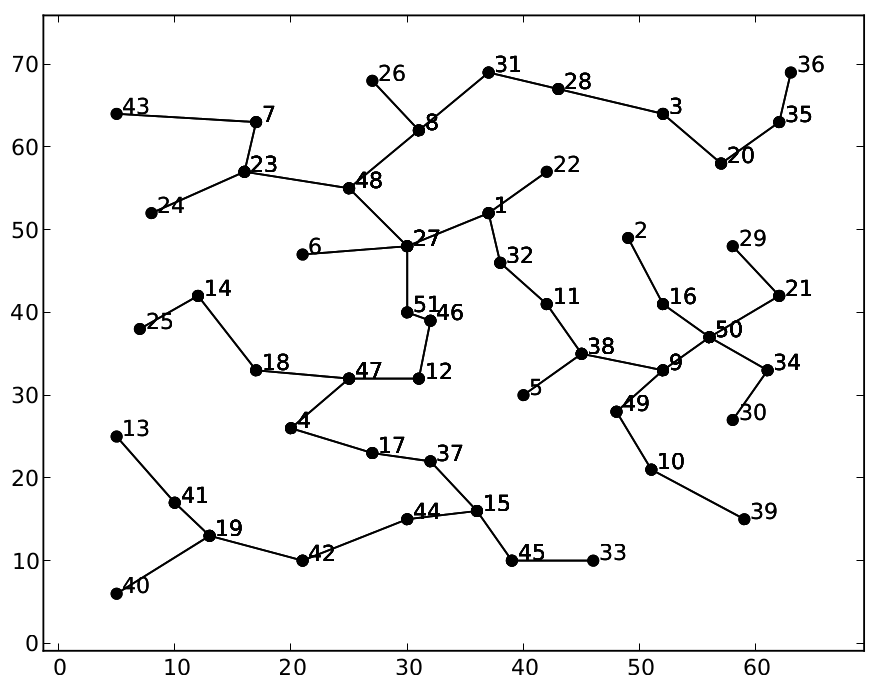
\includegraphics[width=8cm]{gfx/eil51_mst}
            \caption{minimaler Spannbaum}
        \end{figure}
    \end{frame}
    \begin{frame}
        \frametitle{Berechnungen - TSPLIB}
        \begin{figure}[H]
            \centering
            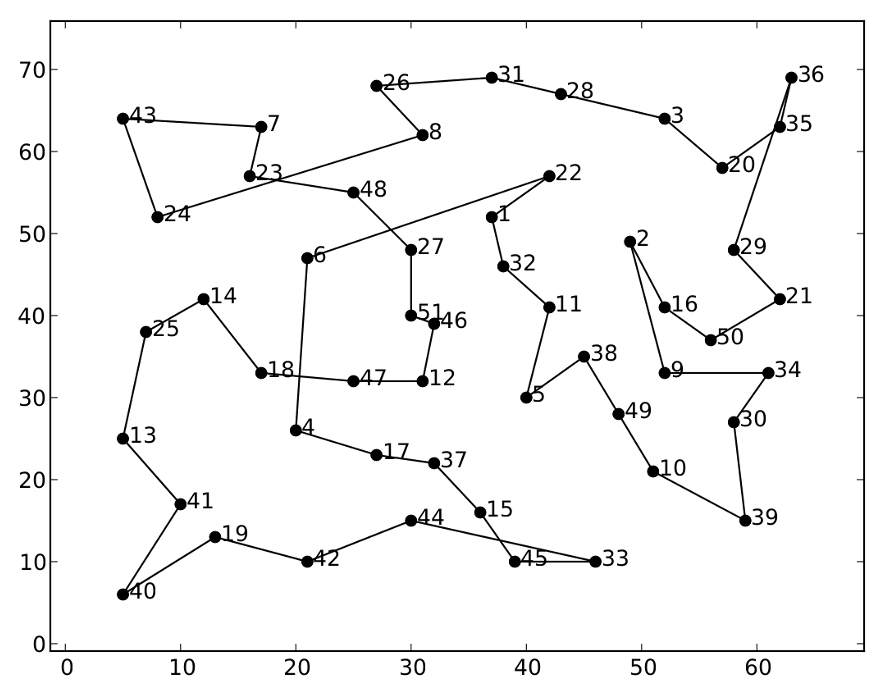
\includegraphics[width=8cm]{gfx/eil51_tour}
            \caption{Win/Win Tour}
        \end{figure}
    \end{frame}
    \begin{frame}
        \frametitle{Berechnungen - TSPLIB}
        \begin{figure}[H]
            \centering
            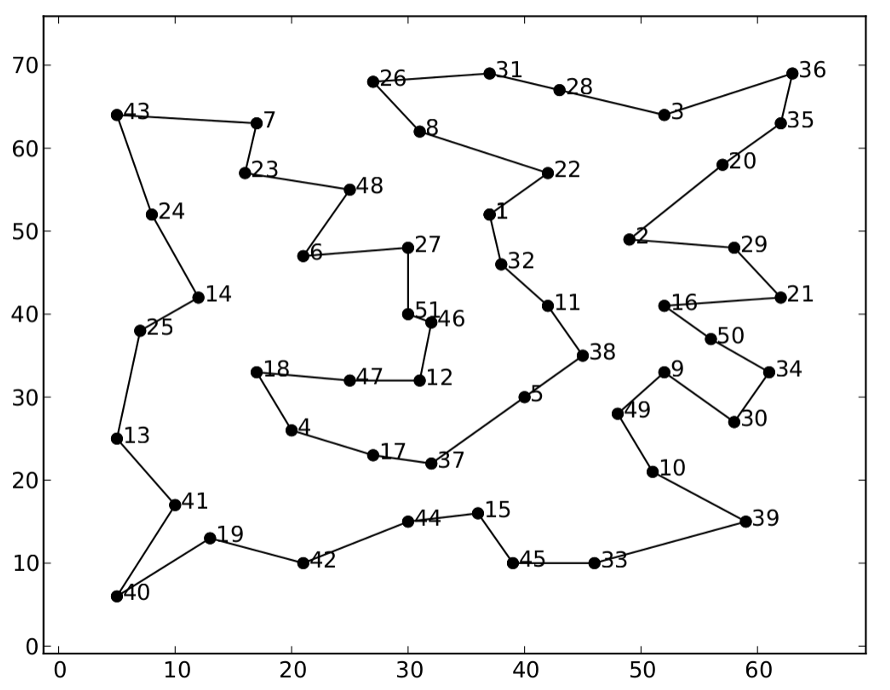
\includegraphics[width=8cm]{gfx/eil51_opt}
            \caption{optimale Lösung}
        \end{figure}
    \end{frame}
    \begin{frame}
        \frametitle{Berechnungen - eigene Instanzen}
	    \begin{itemize}
                \item Worst Case Christofides und Hoogeveen disjunkt
                \item Hoogeveen bei länglichen Instanzen etwas im Vorteil
                \item keine Unterschiede für zufällige Instanzen
            \end{itemize}
    \end{frame}
    \begin{frame}
        \frametitle{Berechnungen - eigene Instanzen}
        \begin{figure}[H]
            \centering
            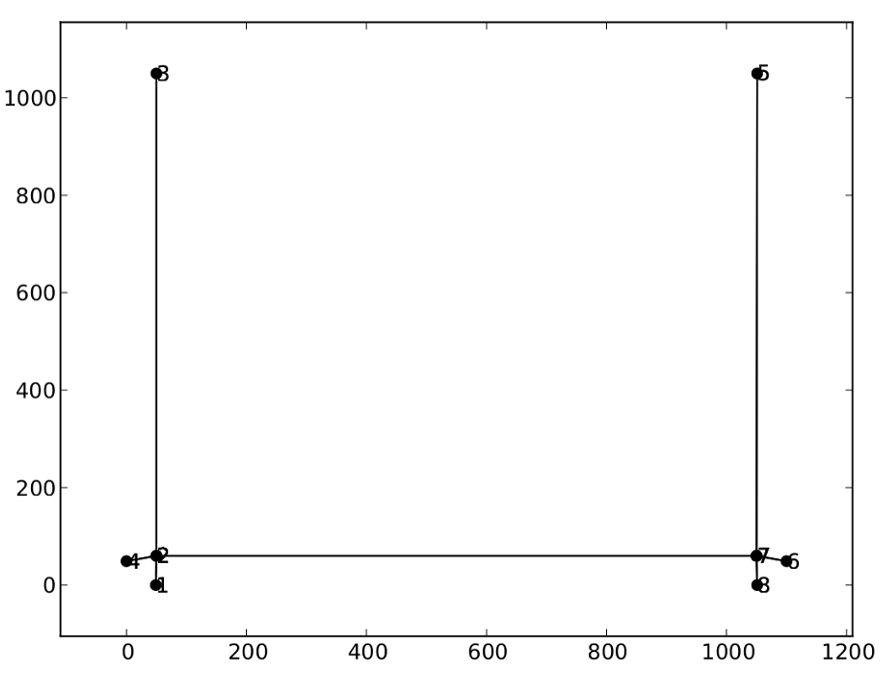
\includegraphics[width=8cm]{gfx/hoogeveen_hpp_mst}
            \caption{minimaler Spannbaum}
        \end{figure}
    \end{frame}
    \begin{frame}
        \frametitle{Berechnungen - eigene Instanzen}
        \begin{figure}[H]
            \centering
            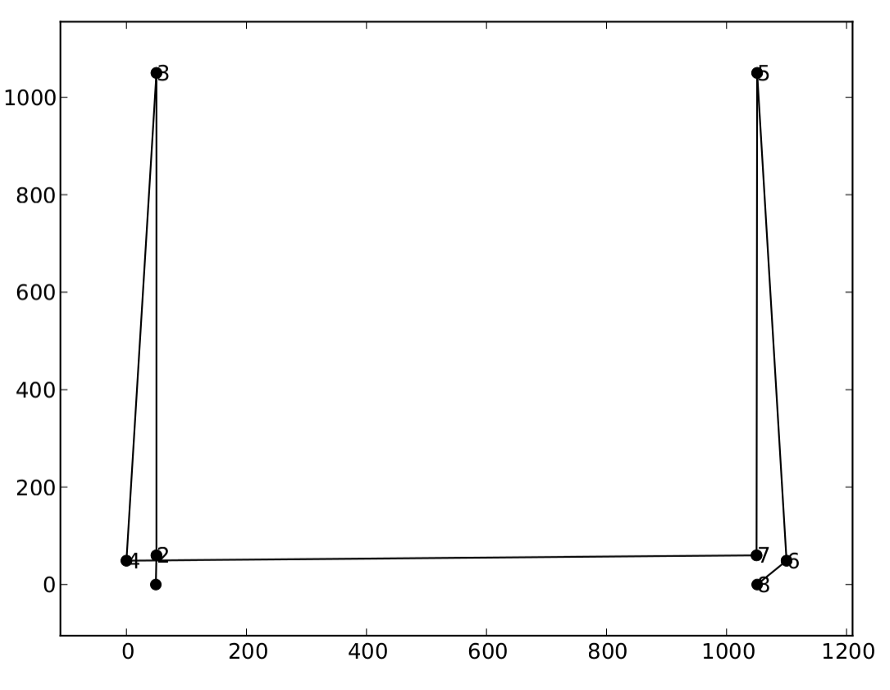
\includegraphics[width=8cm]{gfx/hoogeveen_hpp_tour}
            \caption{Win/Win Tour}
        \end{figure}
    \end{frame}
    \begin{frame}
        \frametitle{Berechnungen - eigene Instanzen}
        \begin{figure}[H]
            \centering
            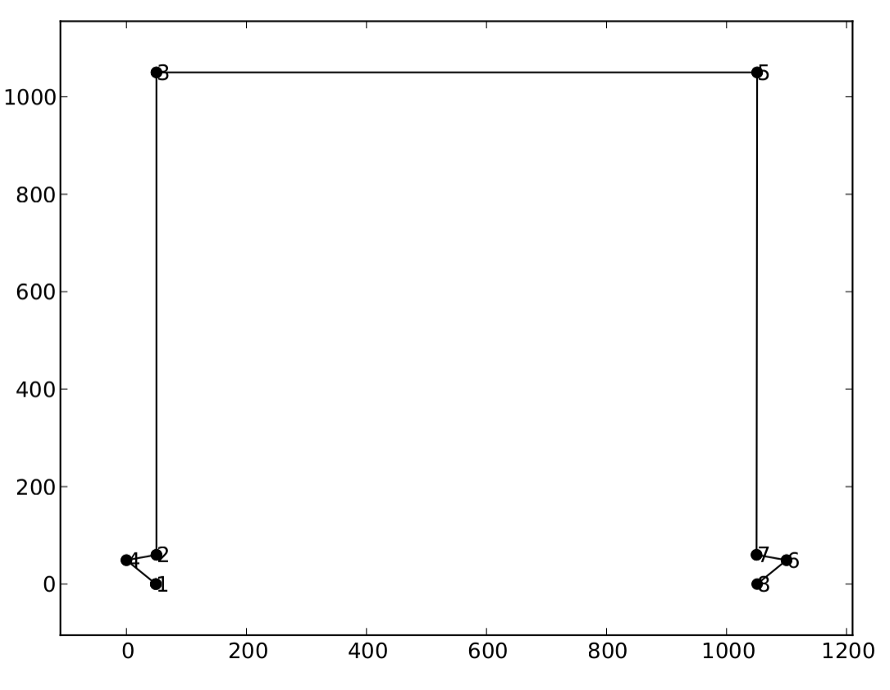
\includegraphics[width=8cm]{gfx/hoogeveen_hpp_optimal}
            \caption{optimale Lösung}
        \end{figure}
    \end{frame}

    \section{Fazit}
    \begin{frame}
        \frametitle{Fazit}
	    \begin{itemize}
                \item Worst Case Instanzen konnten berechnet werden
                \item Allgemein keine Vorteile
                \item obere Grenze wird nur sehr selten erreicht
                \item Abweichung meistens weniger als 15\%
            \end{itemize}
    \end{frame}

    \section{Fragen}
    \begin{frame}
    \frametitle{Fragen}
        \begin{figure}[H]
	    \centering
	        
\includegraphics[width=6cm]{gfx/questionmark}
        \end{figure}
    \end{frame}
\end{document}
